\section{R Code and Data Sources}
\label{ch:codesource}

Much of the code was written from scratch for this project, or is a close to direct translation of the formulas described in papers such as Grigorian's \cite{grigor20}.

\subsection{R packages}

\verb|ggplot2|  \cite{ggplot2} is widely used for easily plotting and visualising the models. \verb|rgdal| \cite{rgdal} allows geospatial \verb|.shp| files to be read into \verb|R|. \verb|raster| \cite{raster} allows this data to be manipulated and plotted. \verb|dplyr| \cite{dplyr}  provides useful data manipulation functions, both for models and geospatial mapping. Statistical models (HoltWinters, ARIMA and Neural Network Regression) were readily implemented from \verb|forecast| \cite{forecast}.

\subsection{Plotting and colour}

wesanderson \cite{wesanderson20}

\begin{figure}[!htb]
\minipage{0.98\textwidth}
  
\includegraphics[width=\linewidth]{wespalette.png} \label{fig:wespalette}
  
\includegraphics[width=\linewidth]{wespalette2.png} \label{fig:wespalette2}
  
\includegraphics[width=\linewidth]{wespalette3.png} \label{fig:wespalette3}
\endminipage
\caption{Wes Anderson Palettes}
\end{figure}


\subsection{Shapefiles}

This data includes the geospatial vector data which can be used to \textit{draw} country (and county) coastlines and borders. 

World country shape data was obtained from \cite{countryshape}, while the more detailed county-level shapefile was downloaded from \cite{countyshape}.



\subsection{Datasets}

\underline{Country-based data:}

Originally used data from \cite{ecdcdata},  but the ECDC switched from a daily to a weekly update from 14 December 2020. Therefore, I have chosen to use the data from  \cite{countrydata}, which has remained daily

\begin{figure}[!htb]
\minipage{0.98\textwidth}
  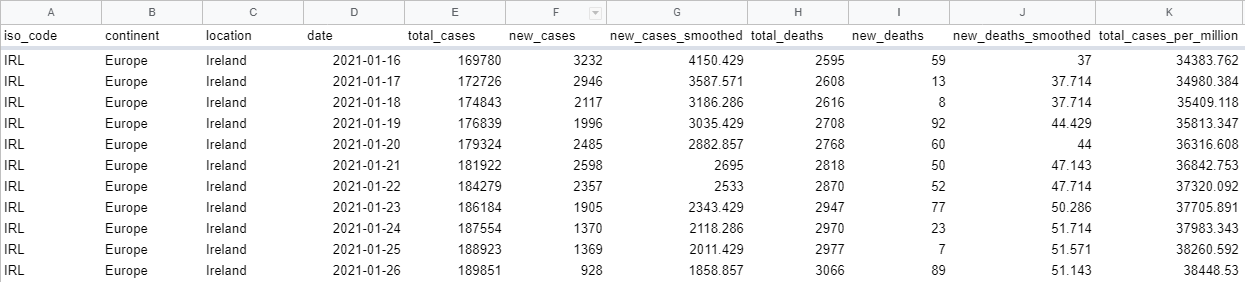
\includegraphics[width=\linewidth]{owiddatextract.png} \label{fig:owiddatextract}
\endminipage
\caption{OWID World data extract}
\end{figure}

\underline{Ireland cases by county}
Downloaded from \cite{irelanddata}.

\begin{figure}[!htb]
\minipage{0.98\textwidth}
  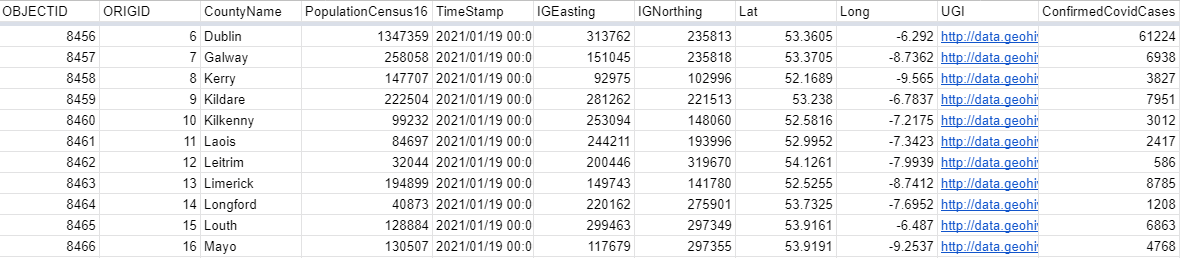
\includegraphics[width=\linewidth]{irelanddatextract.png} \label{fig:irelanddatextract}
\endminipage
\caption{ArcGIS Ireland data extract}
\end{figure}

